\documentclass[11pt,a4paper,titlepage,french]{article}
\usepackage{ifpdf}
\usepackage[utf8]{inputenc}
\usepackage[francais]{babel}
\usepackage[T1]{fontenc}
%\usepackage[top=3cm,right=3.5cm,bottom=3cm,left=3.5cm]{geometry}
\usepackage{graphicx}
\usepackage[unicode=true,pdftex,colorlinks=true,linkcolor=black,urlcolor=black]{hyperref}

\newcommand{\HRule}{\rule{\linewidth}{0.5mm}} %Pour mettre dans la title page
\parindent 1.0cm
\setlength{\parskip}{1em plus 0.5ex minus 0.5ex}

\title{Intelligence Artificielle : Atari Go}
\author{Julien \textsc{Durillon} \and Clotilde \textsc{Massot}}
\date{\today}

%Partie pdf
\ifpdf
\pdfinfo {
	/Author (Julien Durillon - Clotilde Massot)
	/Title (Intelligence Artificielle : Atari Go)
	/Subject (Intelligence Artificielle : Atari Go)
	/Keywords (IA, go, alma)
	/CreationDate (D:20100219175732)
}
\fi
%Fin partie pdf


\begin{document}
%	\maketitle
	\begin{titlepage}

\begin{center}


% Upper part of the page

\includegraphics[scale=1.00]{./logo_fac.png}
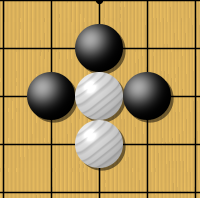
\includegraphics[scale=0.5]{./logogo.png}\\[1cm]

\textsc{\LARGE Intelligence artificielle}\\[1.5cm]

\textsc{\Large Projet TP : Atari Go}\\[0.5cm]


% Title
\HRule \\[0.4cm]
{ \huge \bfseries Étude du jeu et des possibilités d'heuristique}\\[0.4cm]

\HRule \\[1.5cm]

% Author and supervisor
\begin{minipage}{0.4\textwidth}
\begin{flushleft} \large
\emph{Auteurs :}\\[0.2cm]
\end{flushleft}
\end{minipage}

\begin{minipage}{0.5\textwidth}
\begin{flushright} \large
Clotilde \textsc{Massot}\\
Julien \textsc{Durillon}
\end{flushright}
\end{minipage}

\vfill

% Bottom of the page
{\large \today}

\end{center}
\end{titlepage}


	\tableofcontents
	\clearpage

	\listoffigures
	\clearpage

	\abstract{Ce document explique l'étude du cas de l'atari-go dans le cadre du projet d'IA du master 1 ALMA 2010. Y sera utilisée la méthode Alpha-Beta pour gérer l'arbre des possibles.}

	\section*{Introduction}
		Le projet demandé dans ce module d'intelligence artificielle est de développer un programme capable de jouer à l'atari-go. Ce jeu est une modification du jeu de go traditionnel, jeu inventé en chine médiévale. La version d'atari-go que nous allons traiter se joue sur un goban plus petit --- d'une taille de 9x9. Le but est d'être le premier à prendre des pierres à l'adversaire. Quand une prise a été effectuée, le jeu est fini. Nous parlerons de pierres ou groupes \emph{adverses} pour désigner les pierres et groupes de l'adversaire, et \emph{alliés} pour désigner les nôtres --- i.e. ceux joués par le programme.

		Nous commencerons par expliciter notre démarche de développement, puis nous continuerons par décrire le cheminement de notre recherche sur les heuristiques, et finirons en présentant l'implémentation de l'algorithme Alpha-Beta, ainsi qu'une éventuelle interface, et les améliorations apportées et pouvant l'être.

	\section*{Notice utilisateur}

		Pour récupérer les dernières sources du projet~: \url{http://alma-go.googlecode.com/svn/groupeE/trunk/atarigo}

		Pour récupérer la version décrite dans ce document~: % Note ici le tag 1.0 du svn

	\section{Mise en place du projet}
		\subsection{Environnement}
		\subsection{Partage du travail}
			L'étude est faite en binôme, et les classes de description du goban ont été faites de la même façon. Le travail est ensuite partagé comme ceci : Clotilde Massot implémente dans un premier temps l'algorithme Alpha-Beta, tandis que Julien Durillon prépare la partie heuristique --- calcul de groupes de pierres\dots % Expliquer l'interface


	\section{Heuristique}

		\subsection{Un premier jet}
			Un premier indice utilisé pour déterminer l'état d'un jeu est d'identifier les groupes de pierres, calculer leurs libertés, et noter les différents groupes en fonction de ce critère. On s'intéresse au groupe qui a le moins de libertés. Si un groupe ami a 0 liberté, le score est fixé à une valeur très basse --- $-2000$ par exemple. À l'inverse, si un groupe adverse a 0 liberté, le score est fixé à $+2000$.

			Cette méthode va entraîner une tendance à construire des longues chaînes. Il faut donc chercher une heuristique plus fine.

		\subsection{Affiner les cas gagnant ou perdant}
			Un cas gagnant --- resp. perdant --- est à première vue un cas où un groupe adverse --- resp. allié --- n'a plus aucune liberté. Mais il existe d'autres cas où un groupe est dit \emph{mort}, c'est-à-dire qu'il ne peut plus sortir vivant. Un des cas les plus évidents est le cas (c.f. figure \ref{groupemort}) où il ne reste plus qu'une liberté, et que l'adversaire est déjà autour de cette liberté.

			\begin{figure}[hbt]
			\label{groupemort}
			\begin{center}
			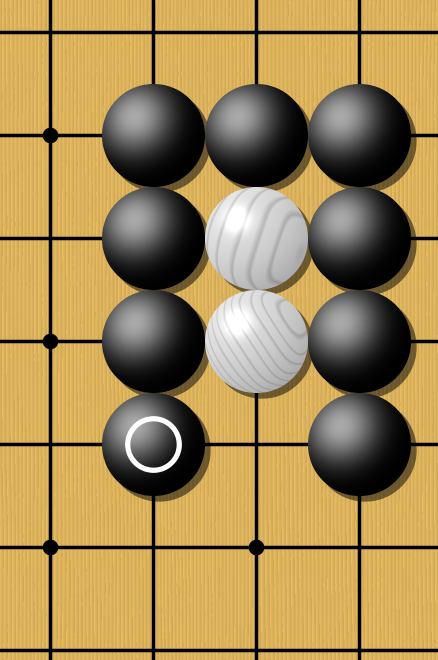
\includegraphics[width=0.4\textwidth]{groupemort.png}
			\end{center}
			\caption{Le groupe blanc est mort}

			\end{figure}

		\subsection{Les yeux}
			Au go, un groupe ayant deux yeux est dit imprenable --- cf. figure \ref{deuxyeux} . Une amélioration de la fonction présentée ci-dessus peut être de détecter de telles dispositions ; en effet, un groupe ayant deux yeux d'une case chacun peut n'avoir que 2 libertés tout en restant imprenable. On noterait alors mieux de tels groupes, et on n'aurait pas à s'en «~soucier~». Pour détecter de tels yeux, il «~suffit~» de chercher des libertés entourées uniquement du bord ou de pierres du groupe étudié. Nous pouvons assez facilement détecter des cas simples d'yeux.

			\begin{figure}[hbt]
			\label{deuxyeux}
			\begin{center}
			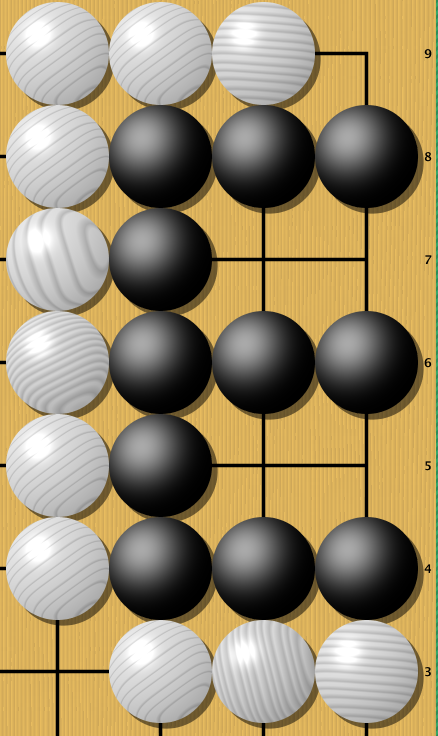
\includegraphics[width=0.4\textwidth]{deuxyeux.png}
			\end{center}
			\caption{Le groupe noir a deux yeux}
			\end{figure}

		\subsection{Les sauts}

			Une des formes intéressantes est le coup en diagonale ou \emph{kosumi} --- cf. figure \ref{kosumi}. Ce coup fait un lien entre les deux pierres qui n'existe pas encore, mais qui ne peut être coupé en un seul coup. Dans la figure \ref{kosumi}, si blanc joue dans le cercle, noir connecte dans le triangle, et vice-versa.

			\begin{figure}[hbt]
			\label{kosumi}
			\begin{center}
			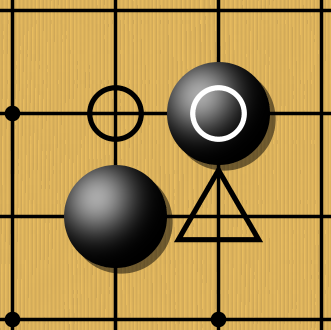
\includegraphics[width=0.3\textwidth]{kosumi.png}
			\end{center}
			\caption{Kosumi}
			\end{figure}

	\section[Algorithme alpha beta]{Algorithme $\alpha\beta$}
	\label{alphab}
		\subsection{Base}
			Cet algorithme se base sur l'algorithme du min-max. La base du min-max consiste à jouer un certain nombre de coups, créer un arbre représentant les possibilités de jeu, donner un score aux états de jeu atteints après génération des coups, et trouver la branche la plus intéressante. Plus un score est haut, plus le jeu est avantageux pour nous. Le parcours de l'arbre est fait en profondeur.

			Pour trouver quelle branche jouer, l'algorithme prend alternativement la branche qui a un score maximum et celle qui a un score minimum, parmi les coups possibles. Si le coup testé est joué par l'IA, la valeur maximum est choisie, car l'IA cherche à jouer le meilleur coup. Si le coup testé est joué par l'adversaire, le minimum est choisi, car l'IA considère que l'adversaire jouera le coup le pire.

		\subsection[Amélioration]{Amélioration $\alpha\beta$}

				L'algorithme du min-max effectue l'évaluation de tous les nœuds de l'arbre de jeu d'un horizon donné. Or dans certains cas --- qui ne sont pas négligeables ---, l'évaluation de certains nœuds n'apporte aucun changement au processus de décision. La figure \ref{abex} va illustrer l'exemple suivant.

				\begin{figure}[hbt]
					\label{abex}
					\begin{center}
						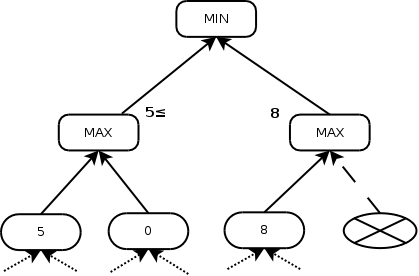
\includegraphics[width=\textwidth]{./alphabeta.png}
					\end{center}
					\caption{Exemple d'élagage $\alpha\beta$}
				\end{figure}

				L'algorithme a calculé la valeur du nœud MAX de gauche, ce nœud prend alors la valeur 5. Lorsque le deuxième nœud max est calculé, on s'aperçoit que la première valeur renvoyée --- en l'occurrence 8 --- est supérieure à 5. Or, comme l'algorithme se trouve dans un cas où il choisira la valeur maximum, le nœud MAX de gauche aura au moins la valeur 8. Donc ce n'est pas la peine d'étudier les sous-arbres suivants, car de toutes façons, c'est le 5 qui sera remonté au niveau d'au dessus.

				L'algorithme $\alpha\beta$ consiste à détecter ces cas de coupure, et donc à éviter des calculs inutiles.


		\subsection{Autres améliorations de l'algorithme}

			\subsubsection{Plusieurs fonctions d'évaluation}
				Pour améliorer cet algorithme, nous allons définir deux fonctions d'évaluation du jeu~:

				\paragraph{evaluateBeginning}
					Cette première fonction est appelée tant que moins de 6 coups ont été joués. Le grand principe de cette évaluation est de s'assurer que les coups sont plutôt joués vers le centre du goban. Comme il n'y a pas encore de groupe, ce n'est pas la peine de calculer les yeux des groupes, et moins important de compter les libertés car il est plus difficile d'être pris au début du jeu.


				\paragraph{evaluateFollowing}
					La deuxième fonction est appelée quand le jeu a déjà bien démarré. Ici sont testés les yeux des groupes, leurs libertés, et les sauts possibles.

			\subsubsection{Réduction des coups possibles}
				Nous considérons que certains coups n'apportent rien. Au début du jeu, on restreint les endroits où jouer au carré central, excluant les deux lignes/colonnes extérieures --- cela équivaut à la zone délimitée par les hoshi. Pendant la suite du jeu, les possibilités  sont encores restreintes à un rectangle entourant les pierres déjà jouées agrandi de deux lignes et colonnes. Le rectangle bleu de la figure \ref{rectangletest} montre la zone qui sera testée dans le cas présenté --- les intersections situées sur les côtés du rectangle sont inclues dans la zone.

				\begin{figure}[hbt]
					\begin{center}
						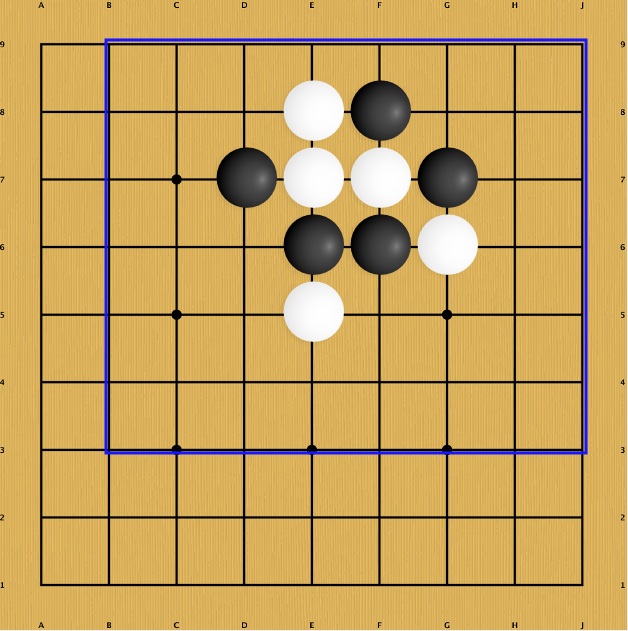
\includegraphics[width=0.7\textwidth]{./rectangle-test.png}
					\end{center}
					\caption{Zone jouable par l'ordinateur}
					\label{rectangletest}
				\end{figure}


			\subsubsection{Arrêt de l'algorithme au plus tôt}
				Nous avons ajouté une pondération de l'évaluation. Si on évalue une feuille qui est à un niveau inférieur au niveau maximum demandé, l'évaluation vaudra plus cher que si la feuille est à la profondeur maximale. Il vaut mieux jouer un très bon coup qui finit le jeu plus tôt qu'un très bon coup qui le finit plus tard.


	\section{Fonctionnement de l'application}

		\subsection{Cas d'utilisation}
			Les cas d'utilisation sont présentés dans la figure \ref{use case}.

			\begin{figure}[ohbt]
				\begin{center}
					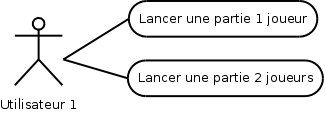
\includegraphics[width=0.7\textwidth]{./usecase.png}
				\end{center}
				\caption{Cas d'utilisation}
				\label{use case}
			\end{figure}

		Les actions possibles ne sont pas foule, car nous avons principalement orienté notre travail sur l'intelligence artificielle de l'application.

		\subsection{Diagrammes de séquence}

			\subsubsection{Partie à un joueur}
				Le déroulement d'une partie à un joueur --- contre l'ordinateur --- est décrit par la figure \ref{oneplayer} --- page \pageref{oneplayer}.

				\begin{figure}[ohbt]
					\begin{center}
						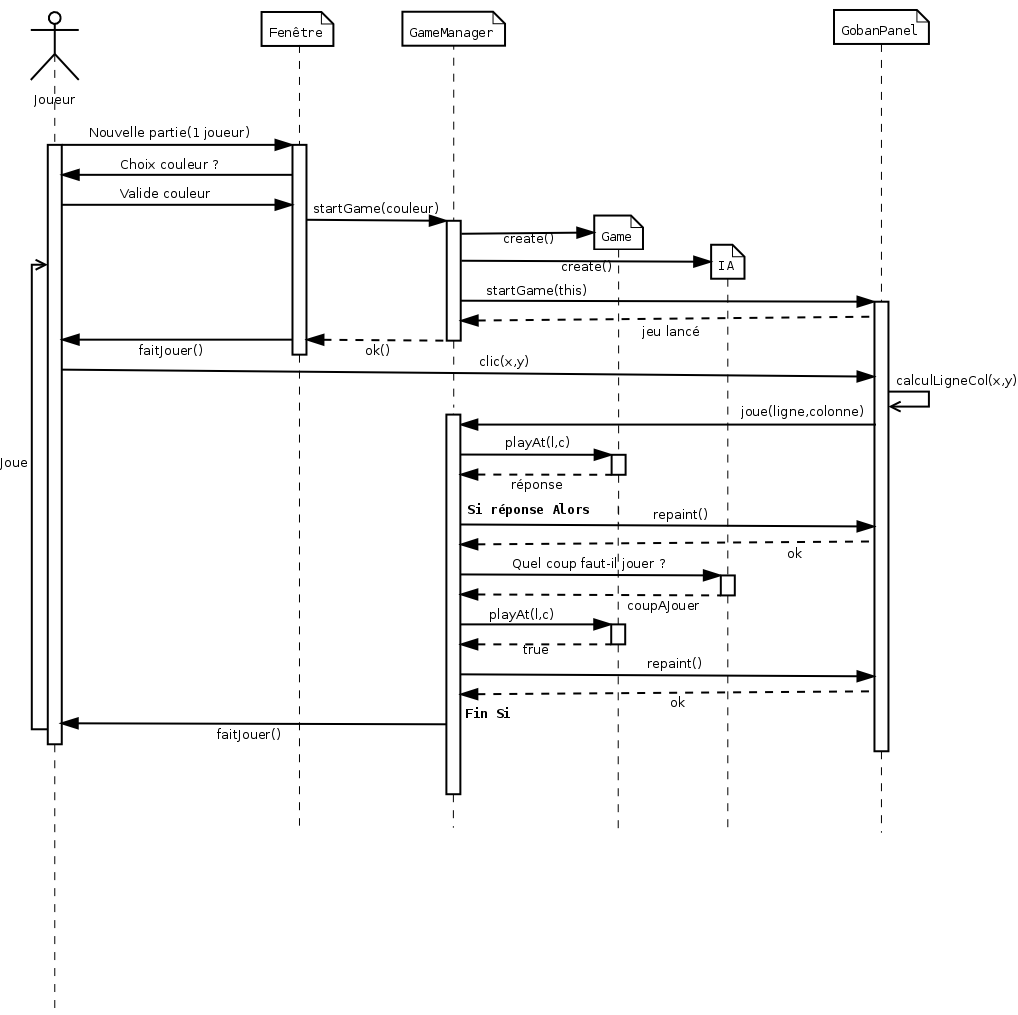
\includegraphics[width=1.1\textwidth]{./IA_1J.png}
					\end{center}
					\caption{Partie à un joueur}
					\label{oneplayer}
				\end{figure}


				Nous pouvons y distinguer des grands éléments de notre application~: la fenêtre principale, le contrôleur --- GameManager ---, le plateau graphique --- GobanPanel ---, le jeu en lui même, et la partie IA --- soit l'algorithme $\alpha\beta$. L'algorithme $\alpha\beta$ a été décrit dans la section \ref{alphab}. Le jeu en lui-même sera décrit dans la section \ref{howgame}. Pour lancer une partie, le joueur doit cliquer sur le bouton idoine. S'il a choisi une partie à un joueur, l'application lui demande la couleur qu'il veut jouer. Une fois la couleur choisie, on alternera les coups joués par l'ordinateur et les coups joués par le joueur.

			\subsubsection{Partie à deux joueurs}

				La figure \ref{twoplayers} (page \pageref{twoplayers}) décrit le déroulement d'une partie à deux joueurs.

				\begin{figure}[ohbt]
					\begin{center}
						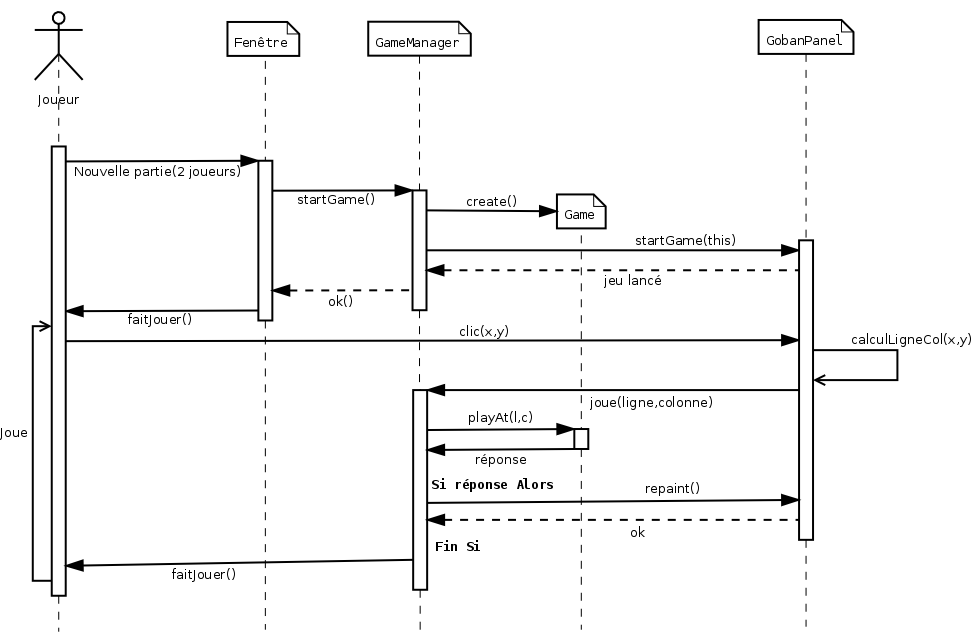
\includegraphics[width=1.1\textwidth]{./IA_2J.png}
					\end{center}
					\caption{Partie à deux joueurs}
					\label{twoplayers}
				\end{figure}

				Si le joueur demande une partie à deux joueurs, on attendra chaque événement de clic sur le jeu et on appliquera le coup.

		\subsection{Le jeu : la classe Game}\label{howgame}


			\subsubsection{Game et Goban}

			Le centre de l'application est ici la classe Game. Elle représente une partie d'atari go. Elle contient le goban courant --- état du plateau ---, un arbre de déroulement de la partie --- prévu pour pouvoir annuler un coup ---, des informations sur les groupes, leurs libertés, etc.

			Le diagramme de classes décrit par la figure \ref{classes} (page \pageref{classes}) montre l'agencement des différents éléments composant un jeu.


				\begin{figure}[hbt]
					\begin{center}
						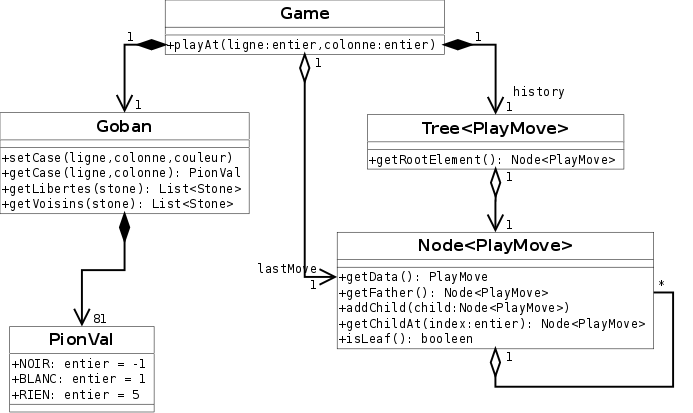
\includegraphics[width=1.1\textwidth]{./classes.png}
					\end{center}
					\caption{Diagramme de classes : Game}
					\label{classes}
				\end{figure}

			Ce diagramme est incomplet. Néanmoins, il permet de repérer les différents éléments d'un jeu. La classe Game en elle-même ne contient qu'une méthode utile pour un joueur~: \emph{playAt}. Les autres méthodes publiques servent pour la fonction d'évaluation et l'algorithme $\alpha\beta$. La classe Goban est une classe métier. Elle contient le plateau tel que représenté logiquement, ainsi que des méthodes d'accès basiques, sans vérification, et des méthodes de récupération des voisins ou des libertés de pions.


			\subsubsection{L'historique}

				L'historique joue un rôle important dans le jeu. Prévu pour suivre le déroulement du jeu, et pouvoir revenir en arrière si besoin, il contient les informations de groupes, de fin de jeu, de modifications à chaque coup du jeu.

				Le diagramme de la figure \ref{history} (page \pageref{history}) décrit sa composition.

					\begin{figure}[hbt]
						\begin{center}
							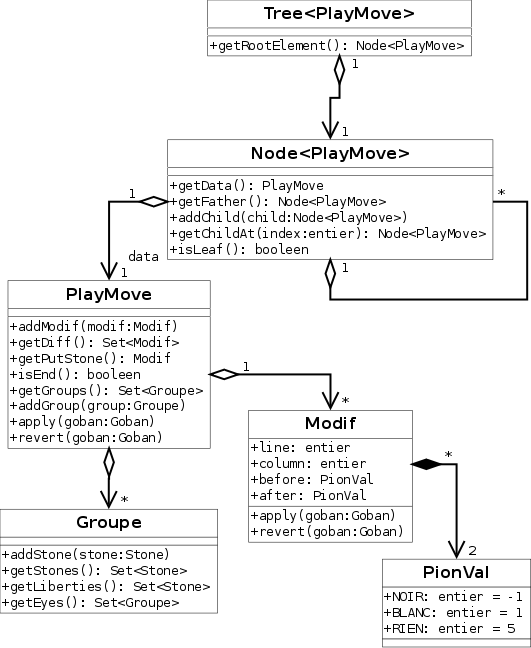
\includegraphics[width=\textwidth]{./history.png}
						\end{center}
						\caption{Diagramme de classes : Historique}
						\label{history}
					\end{figure}

				La partie Historique n'est qu'une structure d'arbre chaîné. La partie importante ici est la notion de PlayMove. C'est cette classe qui contient tous les changements engendrés par le coup qui vient d'être joué. On y trouve~:
				\begin{itemize}
					\item les groupes du moment~;
					\item les changements sur le goban (ajout/suppression de pierres)~;
					\item un booléen en cas de prise, appelé end dans notre cas.
				\end{itemize}

				Les groupes sont des ensembles de pierres. Ils sont décrits dans la section \ref{groupes}. Les changements --- décrits par des objets Modif ---, représentent un diff du goban avant et après le coup. Modif contient des coordonnées, ainsi que la valeur à ces coordonnées avant et après le coup. On ne peut avoir que des couples (RIEN,NOIR), (RIEN,BLANC), (BLANC,RIEN) et (NOIR,RIEN).



			\subsubsection{Les groupes}\label{groupes}

				Les groupes sont des ensembles de pions --- ici Stone. Tous les groupes d'un PlayMove forment une partition de l'ensemble des pierres présentes sur un plateau. Chaque pierre est dans un unique groupe, et n'y est qu'en un seul exemplaire. Nous utilisons ici l'interface Set, et son implémentation HashSet. Les codes de hashage des objets Stone sont étudiés pour être uniques. Un groupe ne contient évidemment que des pierres de même couleur. Le choix de l'implémentation est justifié par le fait que les opérations de recherche, ajout et supression d'éléments dans un HashSet sont faites en $O(1)$, tant que leurs hashCodes sont vraiment uniques.

	\section*{Conclusion}

		Malgré la lenteur de l'algorithme d'intelligence artificielle, qui ne tient pas vraiment compte de la limite de temps donnée, le jeu est possible. Nous avons pu trouver des améliorations de l'algorithme $\alpha\beta$ pour court-circuiter des évaluations inutiles. Il aurait peut-être néanmoins été plus intéressant de réaliser ce projet dans un langage plus à même de traiter ce genre de problèmes, tel que le \emph{prolog}.


\end{document}
